\documentclass{beamer}
\usepackage[magyar]{babel}
\usepackage{t1enc}
\usetheme{AnnArbor}
\usepackage{tabularx}
\usecolortheme{default}

\begin{document}
\author{Komjáti Ákos, Balla Tamás}
\title{pdfslide csomag használta}
\subtitle{Bevezetés a \TeX-be}
\date{2021/22/I.\ félév}

\frame[plain]{\maketitle}
%%slide
\begin{frame}{Csomag célja}
\begin{itemize}

\item Egy olyan módszert kidolgozni amivel könnyebb prezentációkat készíteni.\pause

\item Segítse a matematikai formulák szöveggel és grafikák keverésében amire a mai WYSIWYG eszközök nem képesek\pause

\item Hogy kihasználja a \TeX{} platform függetlénségét és így a prezentációk hordozhatóvá válhatnak.\pause

\item Különféle hátterek használatának szabadsága és egyéb díszítések lehetősége.

\end{itemize}
\end{frame}

\begin{frame}[fragile]{Implementálás}
\begin{enumerate}
\item Készítsünk \LaTeX{} dokumentumot a szokásos módon. \pause
\item A preambulumban töltsük be a diacsomagot a \color{red}{\verb|\usepackage{pdfslide}|}\color{black}paranccsal. Ezt az utolsó csomagként kell betölteni. Kötelező a hyperref.sty 6.60-as vagy újabb verziója telepítve legyen a rendszerére. \pause
\item Futtassuk a pdfLATEX-et a dokumentumon, így megkapjuk a pdf kimenetet
amelyet az Acrobat Readerrel tekinthetünk meg.
 
\end{enumerate}
\end{frame}

\begin{frame}[fragile]{Dia készítése}
\begin{itemize}
\item 
Diát \color{red}{\verb|\section{Name}|} \color{black} paranccsal hozhatunk létre ahol a szakasz neve lesz a dia címe
\pause
\item A diákat  \color{red}\verb|\pause| \color{black}paranccsal tördelhetjük  
\end{itemize}
\end{frame}

\begin{frame}[fragile]{Oldalátmenet}
Kihasználhatja az Acrobat oldalátmeneti lehetőségeit.
Specifikusan adja meg ezzel a parancssal
\color{red}\verb|\pagedissolve{<opció>}| \color{black} \\
\textbf{Parancsok az oldalátmenet} \\
\begin{table}[h]
\begin{tabularx}{\textwidth}{l X}
\verb|/split| & Két sor söpör végig a képernyőn, hogy felfedje az új oldal hasonló függönyt nyitni. \\
\verb|/blinds| & Hasonló a \verb|/Splithez|, de több sorral, amelyek hasonlítanak a „redőnyökhöz” \\

\verb|/box|& A régi oldal közepétől egy doboz megnagyobbodik, hogy felfedje az újat \\

\verb|/wipe|& Egyetlen sor „áttörli” a régi oldalt, hogy felfedje az újat. \\

\verb|/dissolve|& A régi oldal „feloldódik”, hogy felfedje az újat. \\

 \verb|/glitter|& Hasonló a \verb|/Dissolve|-hoz, kivéve, hogy az effektus egyik élről a másikra söpör. \\

\verb|/R|&  A régi oldalt egyszerűen lecserélik az újra, minden különösebb dolog nélkül hatás. Ez az alapértelmezett. \\


\end{tabularx}
\end{table}

\end{frame}


\begin{frame}[fragile]{Hátterek}
\begin{itemize}
\item Létrehozhatunk saját háttérgrafikát amit a \color{red}\verb|\overlay{<fájlnév>}|\color{black} paranccsal meghívhatunk meg őket.
\pause

\item A pdfslide csomag három grafikus fájlformátumot támogat:\textcolor{red}{\tt pdf, jpeg, png}. Az \textcolor{red}{\tt eps} és egyéb nem támogatott fájlokat Ghostscript segítségével konvertálhatjuk pdf formátumba.
\pause

\item Minden egyes oldalnak egyedi hátteret állíthatunk be, nincs ilyen téren
határ.


\end{itemize}
\end{frame}
\begin{frame}
\begin{tabular}{cc}
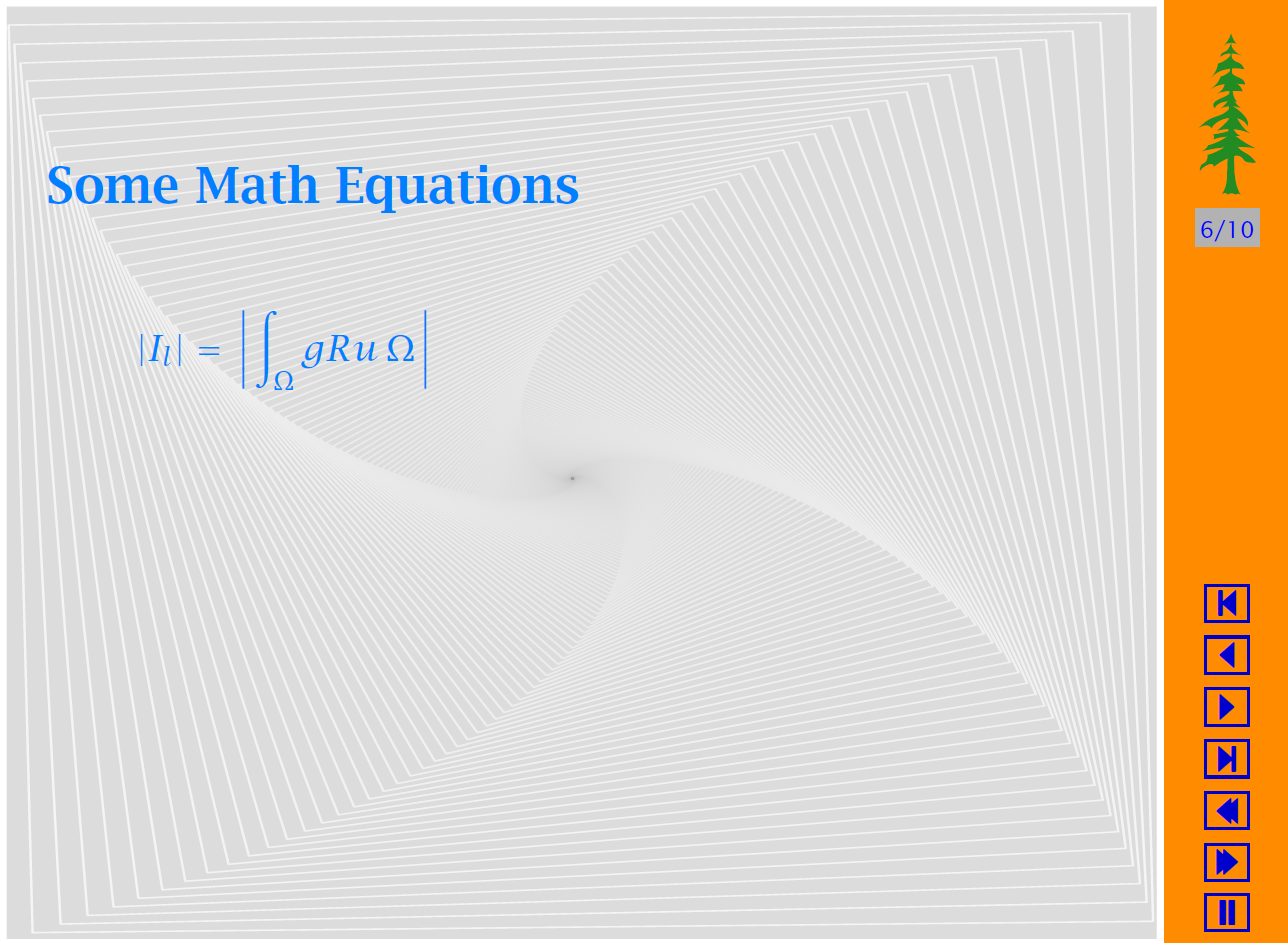
\includegraphics[width=5cm]{egyen1} 1 & 
\includegraphics[width=5cm]{hatter1} 2 \\
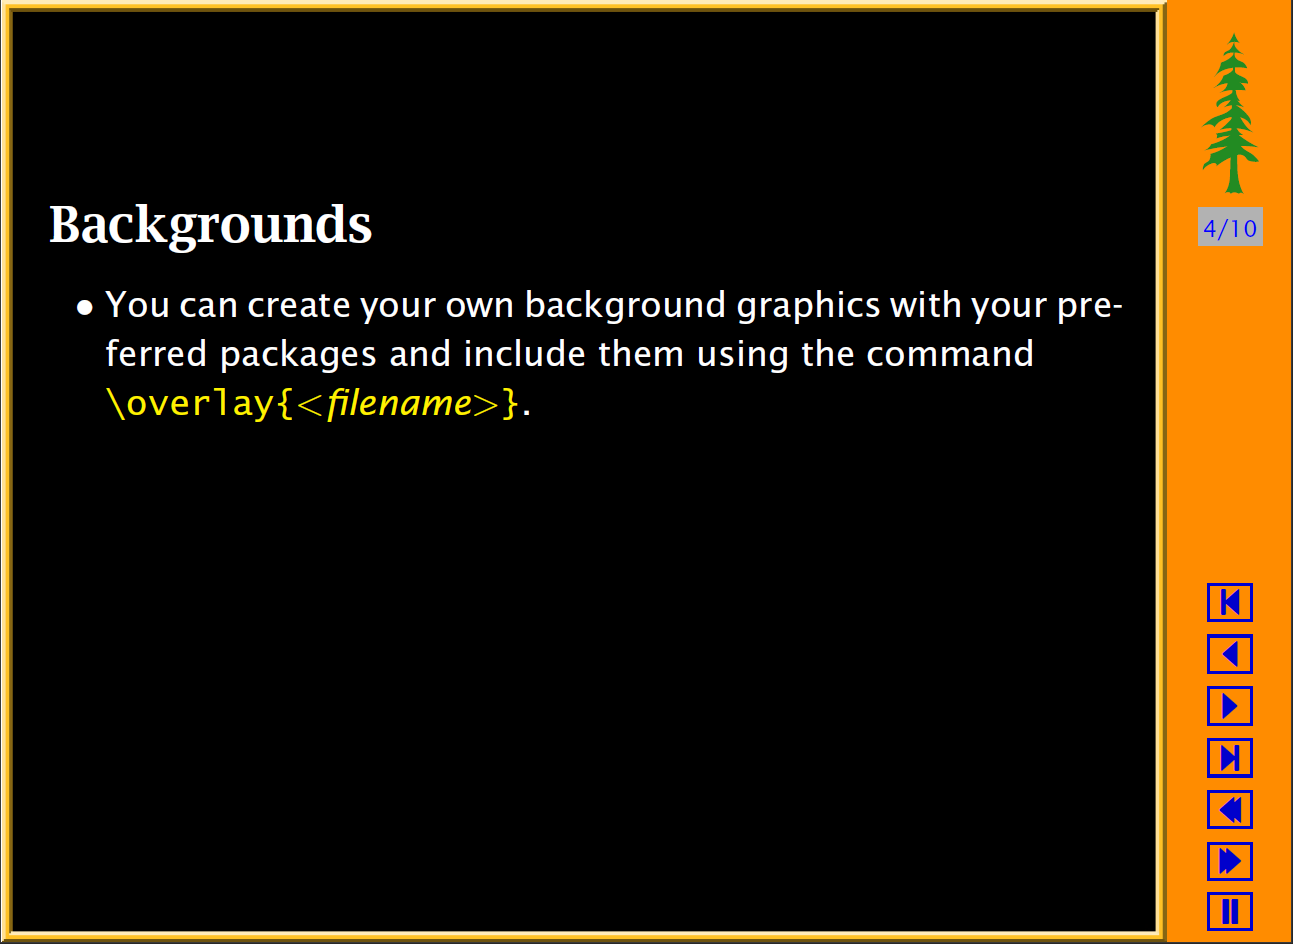
\includegraphics[width=5cm]{hatter2} 3 & 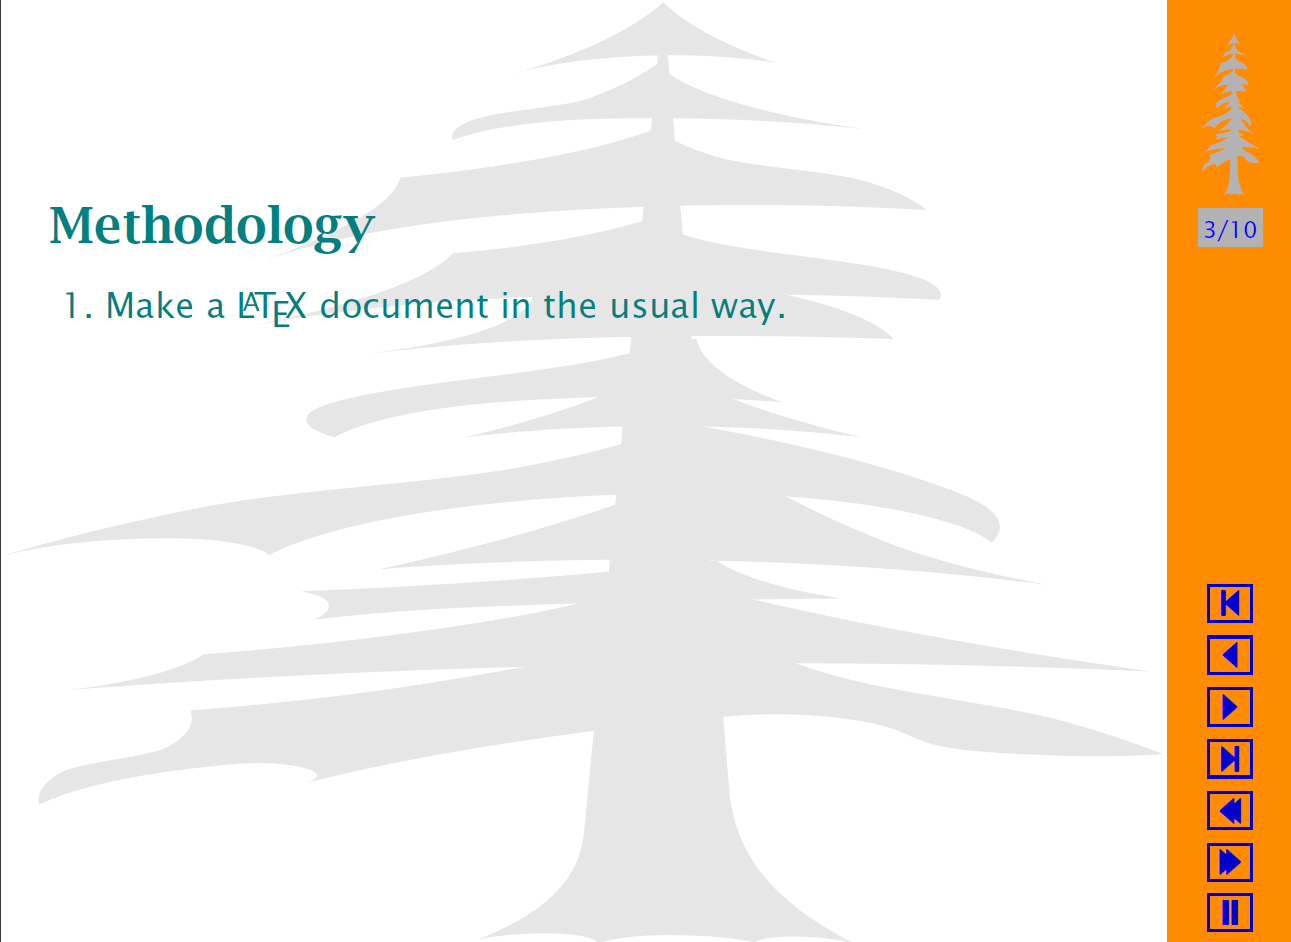
\includegraphics[width=5cm]{hatter3} 3 \\ 
\end{tabular}
\end{frame}

\begin{frame}[fragile]{Egyenletek bemutatása}
\onslide<1-> Egyenletek bemutatására is remekül alkalmas. A matematikai módban megírt egyenlet sorai után \color{red}\verb|\pause| \color{black}parancsot írva soronként jelenik meg az egyenlet. \\
\onslide<2->
\begin{tabular}{cc}
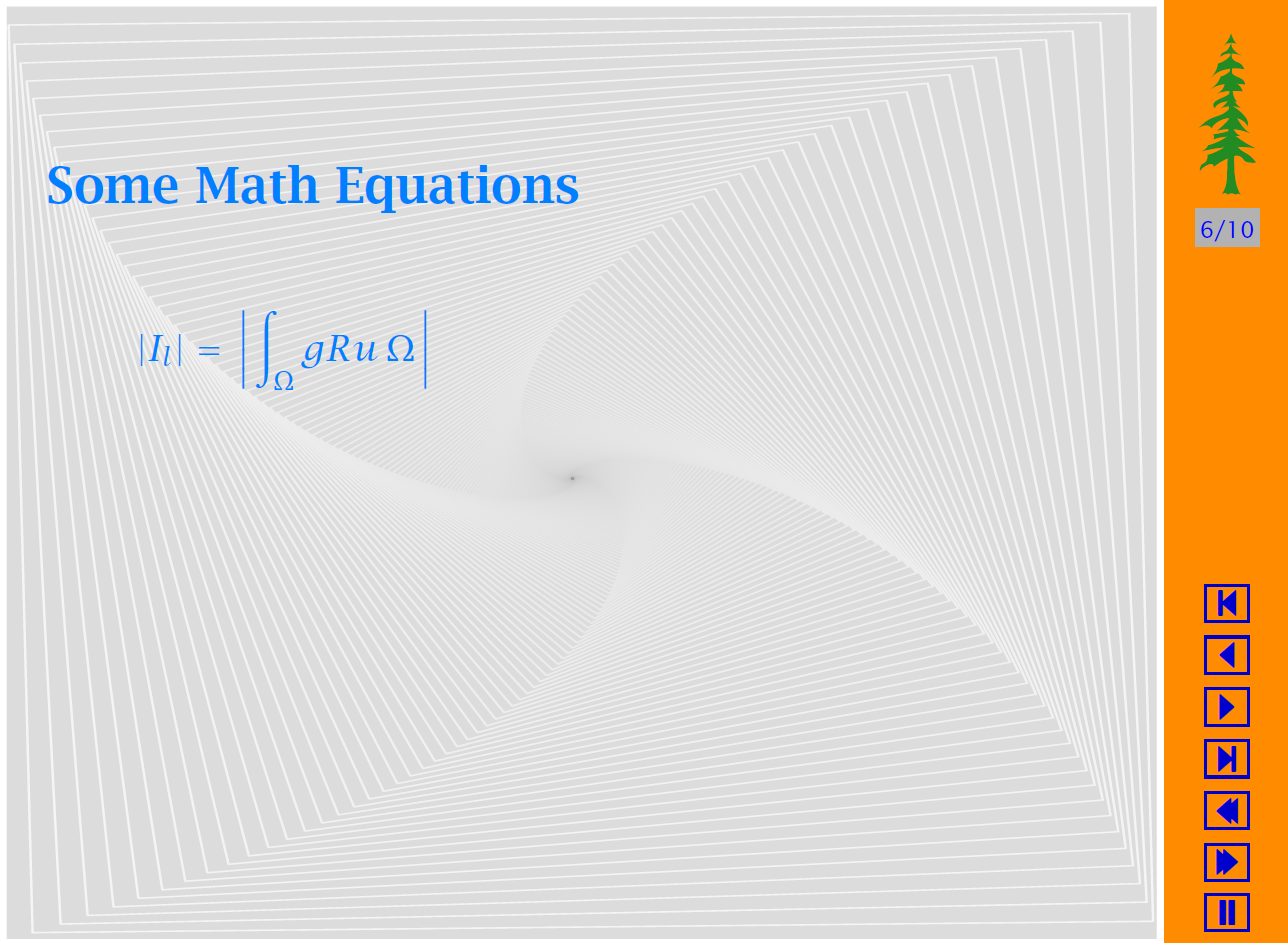
\includegraphics[width=4cm]{egyen1} 1\onslide<3-> & 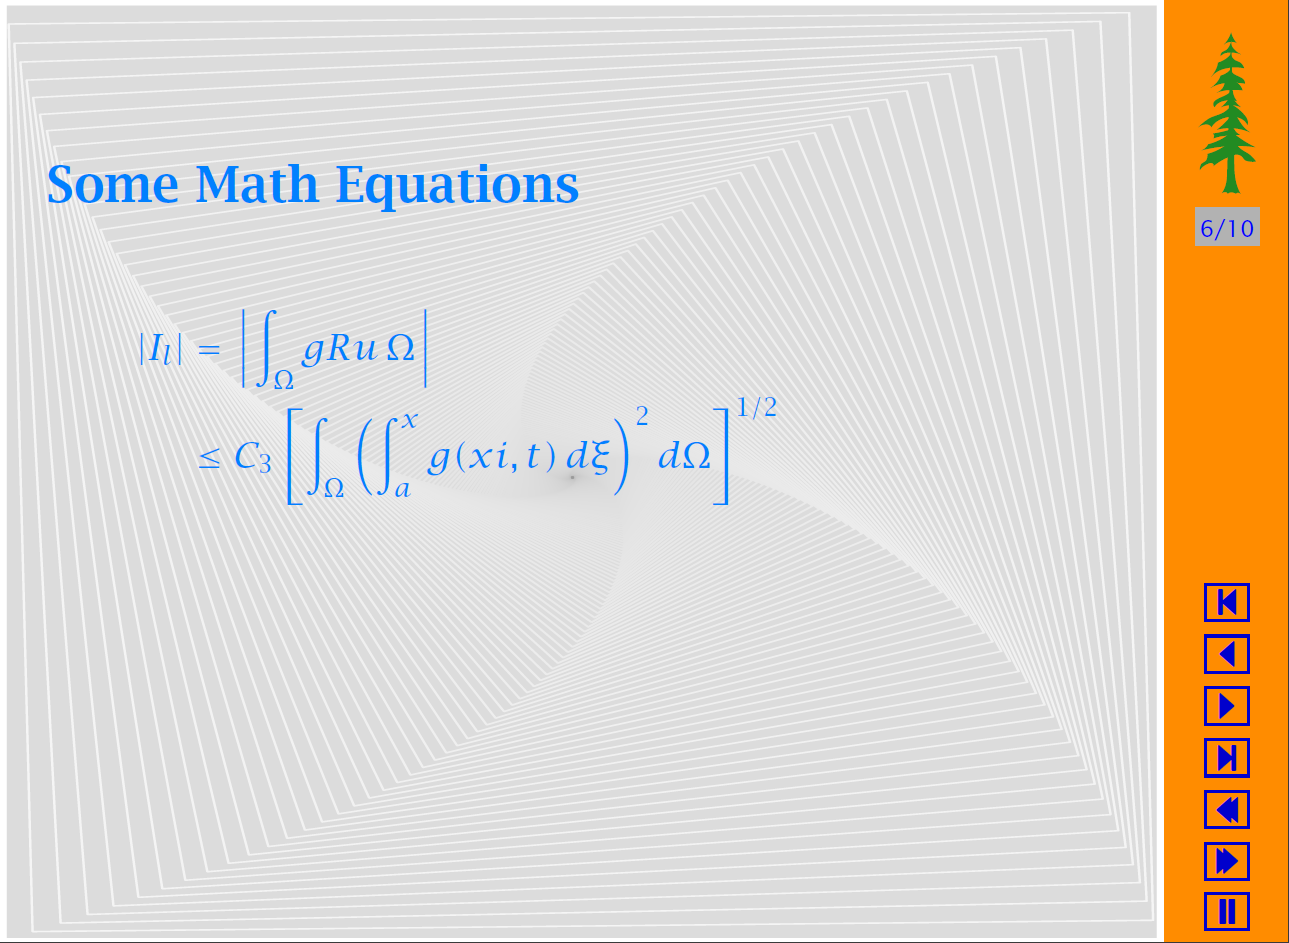
\includegraphics[width=4cm]{egyen2} 2\onslide<4-> \\
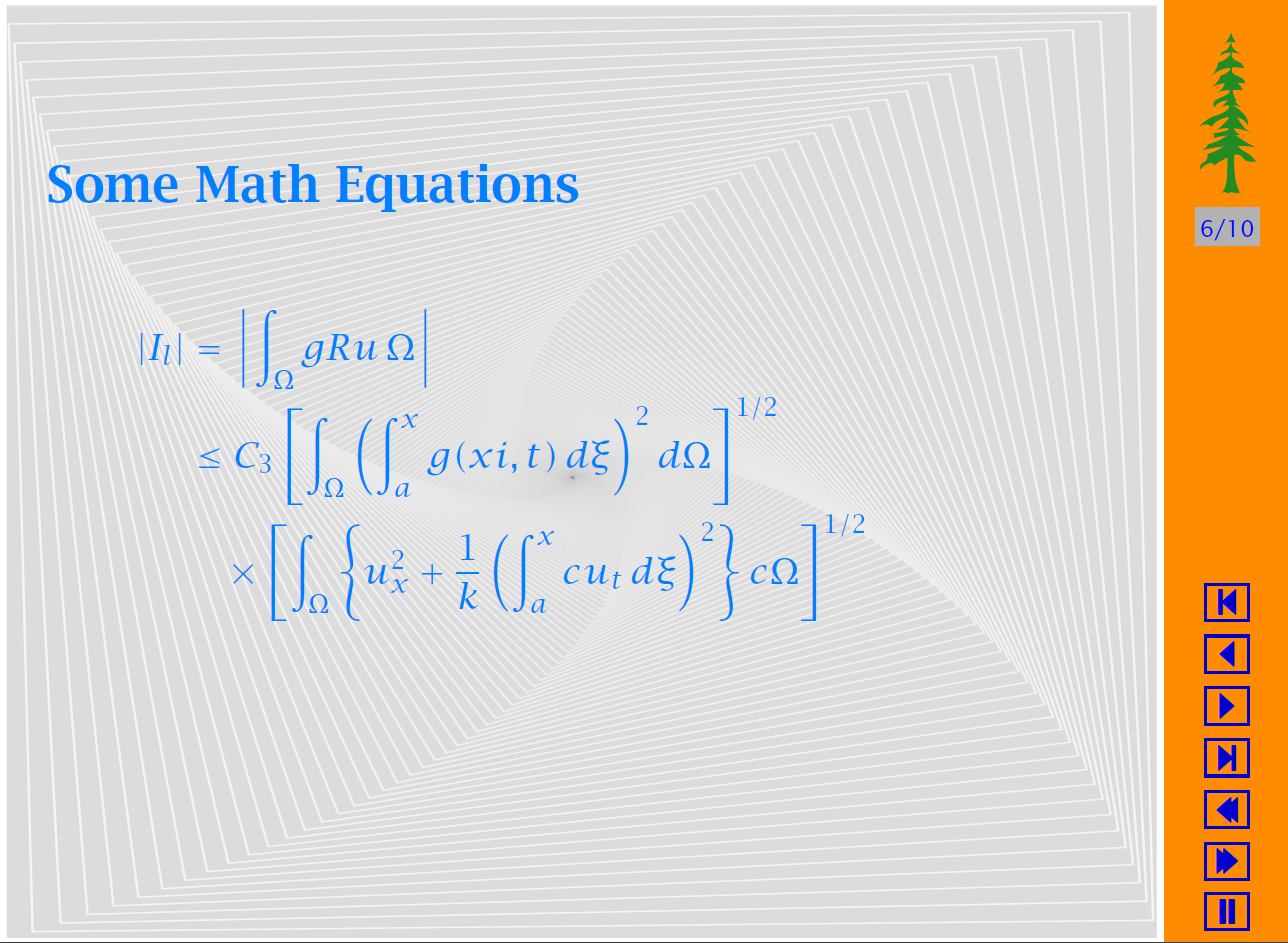
\includegraphics[width=4cm]{egyen3} 3\onslide<5-> & 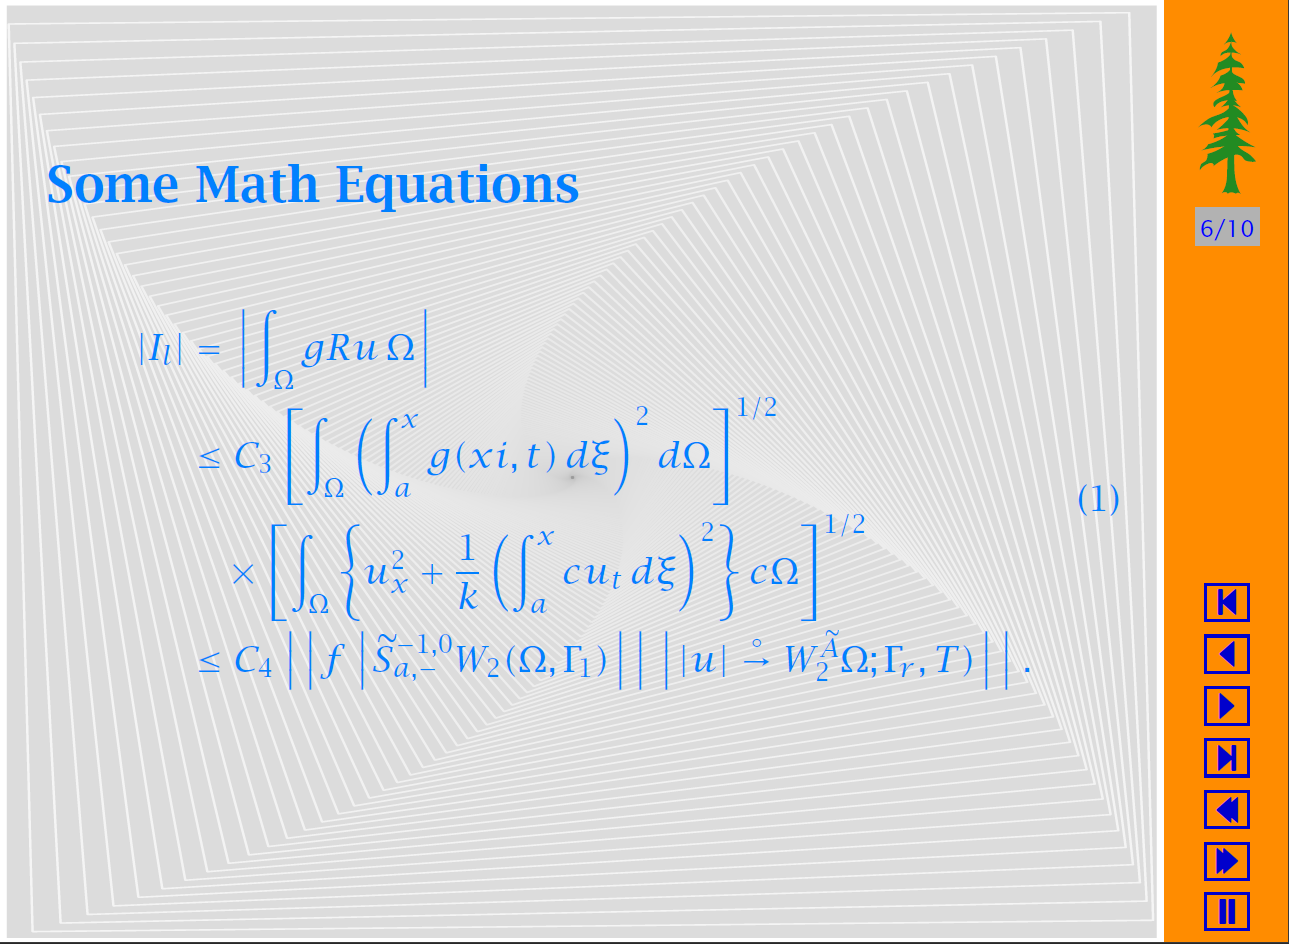
\includegraphics[width=4cm]{egyen4} 3 \\ 
\end{tabular}

\end{frame}

\begin{frame}[fragile]{Egyéb tulajdonságok}
\large \textbf{Betűtípusok} \\
\normalsize
A csomag az összes font attribútumot újra definiálja, hogy nagyobbak legyenek a szokásos méretnél.
Ha azonban vissza akarunk térni az eredeti mérethez, akkor hozzá kell írni a real szót a font size parancs elé, azaz a \color{red}\verb|\normalsize| \color{black}esetén használjuk a \color{red}\verb|\realnormalsize| \color{black}parancsot; \color{red}\verb|\large| \color{black}pedig ez lesz \color{red}\verb|\reallarge| \color{black}és így tovább.

\large \textbf{Címsorok} \\
\normalsize
A \color{red}\verb|\section{...}| \color{black}használható a diák első szintű fejlécére. Ha több hely kihagyásra van szüksége, hagyja ki a címsor előtt, hogy az egész anyagot függőlegesen középre állítsa, módosíthatja a dimenziót a \color{red}\verb|\headskip|={<new dimension>} \color{black} paranccsal. Ez a parancs a szakasz címsora elé kell helyezni, és az aktuális dia végén vissza kell állítani, ha nem szeretné, hogy az aktuális tovább ugorjon.


\end{frame}


\begin{frame}[fragile]{Összefoglalás}
\begin{columns}[T]
\column{0.3\textwidth}
\begin{block}{\color{green}Előnyök}
\begin{itemize}
\item Könnyen használható
\item Személyre szabható háttér
\end{itemize}

\end{block}
\column{0.3\textwidth}
\begin{block}{\color{red}Hátrányok}

\begin{itemize}
\item Nincsenek választható témák
\item Elavult
\end{itemize}
\end{block}

\end{columns}
\end{frame}



%%vége
\begin{frame}
\centering \Large
  \emph{Köszönjük a \\ figyelmet!}
\end{frame}


\end{document}